\documentclass[11pt]{article}
\newcommand{\coursedocname}{Problem Set 2}

\usepackage[utf8]{inputenc}
\usepackage[T1]{fontenc}
\usepackage{lmodern}
\usepackage[margin=1in]{geometry}
\usepackage[dvipsnames]{xcolor}
\usepackage{graphicx, booktabs, enumitem, float, framed, caption, multirow}
\usepackage{fancyhdr}
\usepackage{tcolorbox}
\usepackage{listings}
\usepackage{tikz}
\usepackage{setspace}
\usepackage{needspace}
\IfFileExists{algorithm.sty}{%
  \usepackage{algorithm}
  \usepackage[noend]{algpseudocode}
  \newcommand{\hasalgorithms}{}%
}{}
\usepackage{amsmath,amssymb,bm,xcolor}


\newcommand{\st}{\mathbf{x}}            %

\newcommand{\disc}{\gamma}              %

\newcommand{\loss}{\mathcal{L}}         %
\newcommand{\lr}{\alpha}                %
\newcommand{\params}{\bm{\theta}}       %


\newcommand{\Tf}[2]{{}^{#1}\mathbf{T}_{#2}}  %
\usepackage{hyperref}

\definecolor{DartmouthGreen}{HTML}{00693E}
\newcommand{\dgreen}[1]{\textcolor{DartmouthGreen}{#1}}
\newcommand{\dgbf}[1]{\textbf{\dgreen{#1}}}      %
\urlstyle{same}
\hypersetup{
    colorlinks=true,
    linkcolor=DartmouthGreen,
    filecolor=DartmouthGreen,
    citecolor=DartmouthGreen,
    urlcolor=DartmouthGreen,
    breaklinks=true
}

\newcommand{\coursenumber}{COSC 81/281}
\newcommand{\courseterm}{Fall 2026}
\newcommand{\gradescopelink}{\textbf{Gradescope} (\url{https://www.gradescope.com/courses/1372528})}

\newcommand{\psTwoDue}{Monday, October 5 (11:59pm ET)}

\setlength{\parindent}{0pt}
\setlength{\parskip}{6pt plus 2pt minus 1pt}
\setlength{\headheight}{13.6pt}
\setlength{\emergencystretch}{3em}
\providecommand{\tightlist}{\setlength{\itemsep}{0pt}\setlength{\parskip}{0pt}}
\setcounter{secnumdepth}{0}

\DeclareRobustCommand{\callout}[2][gray!10]{%
  \begin{tcolorbox}[left=8pt, arc=0pt, outer arc=0pt,
                    colframe=#1, colback=#1, coltext=black]#2\end{tcolorbox}}




\newcommand{\gradstar}{$\bigstar$~\textsf{\small (required for 281; optional for 81)}~}
\newcommand{\bonusq}{\textsf{\small\textbf{[Bonus]}}~}
\newcommand{\bonus}{\bonusq}

\newcommand{\setupheader}[1]{%
  \fancypagestyle{default}{%
      \lhead{#1}
      \chead{}
      \rhead{\textbf{\coursenumber}}
      \lfoot{}
      \cfoot{}
      \rfoot{\thepage}
      \renewcommand{\headrulewidth}{0.4pt}
      \renewcommand{\footrulewidth}{0.4pt}
  }
  \pagestyle{default}
  \fancypagestyle{plain}{\pagestyle{default}}
}
\newcommand{\setupexamheader}[1]{%
  \fancypagestyle{default}{%
      \lhead{#1}
      \chead{Name:}
      \rhead{}
      \lfoot{}
      \cfoot{}
      \rfoot{\thepage}
      \renewcommand{\headrulewidth}{0.4pt}
      \renewcommand{\footrulewidth}{0.4pt}
  }
  \pagestyle{default}
  \fancypagestyle{plain}{\pagestyle{default}}
}
\newcommand{\pstitle}[2]{%
  \title{\textbf{\coursenumber:} #1}
  \author{\textbf{Due} #2\\
  }
  \date{}
}

\newcommand{\coursenotice}{%
  \callout{Problem sets are graded \textbf{pass/fail on completion}, and
  there are no late days. The problem sets are where the learning happens,
  and they are the best available practice for the midterm and final exam.
  Submit to \gradescopelink\ and assign each question to a page in your
  submission. Questions are welcome on \dgbf{Slack}. Starred ($\bigstar$)
  questions are required for COSC 281 students and optional (ungraded) for
  COSC 81 students.}}

\lstset{
  language=python,
  basicstyle=\ttfamily,
  commentstyle=\color{BrickRed},
  stringstyle=\color{ForestGreen},
  showstringspaces=false,
  breaklines=true,
  breakatwhitespace=true,
  keywordstyle=\color{Purple},
  emph={def},
  emphstyle=\color{RoyalBlue}
}
\lstnewenvironment{itemlisting}[1][]
 {\mbox{}\vspace*{-\baselineskip}%
  \lstset{xleftmargin=\leftmargin, linewidth=\linewidth, #1}}
 {}

\makeatletter
\def\fps@figure{htbp}
\makeatother
\ifdefined\hasalgorithms
\fi

\newcommand{\docfooter}{\vfill\begin{tiny}Updated \today\end{tiny}}

\newenvironment{studentanswer}[1]
  {\par\medskip\noindent
   \begin{tcolorbox}[height from=#1 to 100cm, colback=white, colframe=gray!60,
     boxrule=0.6pt, arc=0pt, outer arc=0pt, left=7pt, right=7pt,
     top=7pt, bottom=7pt, title={Answer / work}, fonttitle=\small,
     coltitle=black, colbacktitle=gray!8, titlerule=0pt]
   \ignorespaces}
  {\end{tcolorbox}\par}

\setupheader{\coursenumber\ -- \courseterm\ -- \coursedocname}
\pstitle{Problem Set 2: Learning, Optimization, and Control}{\psTwoDue}

\begin{document}
\maketitle

\coursenotice

\begin{quote}\small\textbf{AI Policy.} You may use any AI tools you like to assist you with your assignments, and you should, as that is likely how you will work for the rest of your career.
That being said, the written portions are practice for the in-class midterm and exam, which are closed book and on paper. You should strive to answer these yourself and use AI as a tutor and not an oracle.
\end{quote}

\callout{Please include an AI Tool Disclosure Below \vspace{50pt}}

\raggedbottom
\section*{Overview}

This problem set covers forward kinematics, learning from experience,
gradient descent, and configuration space. Implement gradient descent
and examine its sensitivity to the learning rate. Complete P1--P6 and
the programming task. Starred subparts are required for COSC 281 students
and optional, ungraded practice for COSC 81 students.

\textbf{What to submit.} Submit to \gradescopelink:\vspace{-10pt}
\begin{enumerate}\tightlist
\item \textbf{Written work (PDF)}: your answers to Part 1 and every plot,
      measurement, and short response requested in Part 2. You may write on
      this handout or compile \texttt{ps2/handout.tex}, placing answers and
      figures in its \texttt{studentanswer} environments. Typed boxes expand
      as needed. Assign each question to its page or pages when you upload.
\item \textbf{Code}: \texttt{gd.py}. Before submission, run the public
      checks from the repository root.
      \par\smallskip
      \texttt{python ps2/code/autograder.py}
\end{enumerate}

\clearpage
\section{Part 1: Written problems}

Show your work in each response area. No programming is needed for Part 1.

\subsection*{P1: Forward kinematics of a two-link arm}
A planar arm lies in the world $xy$-plane, with link lengths 2 and 1.
The first joint angle is $90^\circ$ about $+z$; the second is
$-90^\circ$ relative to the first link. Frame 0 is the world frame.
Frame 1 has its origin at the base and its $x$-axis along the first
link. Frame 2 has its origin at the elbow and its $x$-axis along the
second link. The diagram shows the configuration, not additional data.
\begin{center}
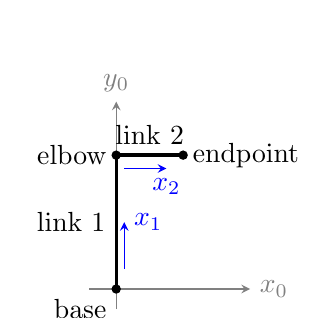
\begin{tikzpicture}[scale=0.85,>=stealth]
\draw[->,gray] (-.4,0)--(2,0) node[right] {$x_0$};
\draw[->,gray] (0,-.3)--(0,2.8) node[above] {$y_0$};
\draw[very thick] (0,0)--(0,2) node[midway,left] {link 1};
\draw[very thick] (0,2)--(1,2) node[midway,above] {link 2};
\fill (0,0) circle(2pt) node[below left] {base};
\fill (0,2) circle(2pt) node[left] {elbow};
\fill (1,2) circle(2pt) node[right] {endpoint};
\draw[->,blue] (.12,.3)--(.12,1) node[right] {$x_1$};
\draw[->,blue] (.12,1.8)--(.75,1.8) node[below] {$x_2$};
\end{tikzpicture}
\end{center}
The notation $\Tf{a}{b}$ maps coordinates from frame $b$ into frame $a$.
Use column vectors and the supplied homogeneous transforms:
\[
\Tf{0}{1}=\begin{bmatrix}0&-1&0&0\\1&0&0&0\\0&0&1&0\\0&0&0&1\end{bmatrix},
\qquad
\Tf{1}{2}=\begin{bmatrix}0&1&0&2\\-1&0&0&0\\0&0&1&0\\0&0&0&1\end{bmatrix}.
\]
\begin{enumerate}[label=(\alph*)]
\item Compute $\Tf{0}{2}$ and the world coordinates of the endpoint,
whose frame-2 homogeneous coordinates are $(1,0,0,1)^\top$.
\begin{studentanswer}{3.5cm}
%%%%% SOLUTION HERE %%%%%
\end{studentanswer}
\item Explain why $\Tf{1}{2}\Tf{0}{1}$ is not the required composition.
Refer to the input and output frames, not only to noncommutativity.
\begin{studentanswer}{2.3cm}
%%%%% SOLUTION HERE %%%%%
\end{studentanswer}
\end{enumerate}

\clearpage
\subsection*{P2: Learning the value of a fixed policy}

A robot follows a fixed policy $\pi$. Two recorded episodes are shown
below. Each arrow is labeled by the reward received on that transition;
$T$ is terminal and $V^\pi(T)=0$. Use $\gamma=\tfrac12$.
\[
\text{Episode 1: } A\xrightarrow{\;0\;} B\xrightarrow{\;4\;}T,
\qquad
\text{Episode 2: } A\xrightarrow{\;0\;} B\xrightarrow{\;2\;}T.
\]
The policy remains fixed throughout this question. Direct evaluation
estimates a state's value by averaging the observed discounted returns
from that state. Temporal-difference (TD) evaluation instead updates
after each transition using
\[
\text{sample}=r+\gamma V^\pi(s'),\qquad
V^\pi(s)\leftarrow(1-\alpha)V^\pi(s)+\alpha\,\text{sample}.
\]
For a transition into $T$, the sample is just $r$.

\begin{enumerate}[label=(\alph*)]
\item \begin{minipage}[t]{\linewidth}
Compute the discounted return from $A$ and from $B$ in each episode.
Then compute the \textbf{direct-evaluation} estimates of $V^\pi(A)$ and $V^\pi(B)$.

\begin{studentanswer}{3.5cm}
%%%%% SOLUTION HERE %%%%%
\end{studentanswer}

\end{minipage}

\item \begin{minipage}[t]{\linewidth}
Initialize both state values to zero and use $\alpha=\tfrac12$ to do \textbf{TD learning}.
Process Episode 1 followed by Episode 2, in the order shown.
For each of the four transitions, record the sample and the updated
value of the state being left. Use the current estimates at each step.

\begin{studentanswer}{4cm}
%%%%% SOLUTION HERE %%%%%
\end{studentanswer}

\end{minipage}

\item \begin{minipage}[t]{\linewidth} \gradstar
Explain why the TD estimates need not equal the direct-evaluation
estimates after these two episodes. Does either calculation establish
that $\pi$ is optimal? Explain in at most three sentences.

\begin{studentanswer}{3.5cm}
%%%%% SOLUTION HERE %%%%%
\end{studentanswer}

\end{minipage}
\end{enumerate}

\clearpage
\subsection*{P3: Exploration and observed rewards}

A tabular Q-learning agent operates on a large grid. The goal is 22
steps from the start and gives reward $+100$ on entry, ending the episode.
A charging pad adjacent to the start gives reward $+1$ each time it is
entered. All other rewards are zero. Episodes end after at most 50 steps,
$\disc=0.9$, $\lr=0.5$, and the Q-table is initialized to zero. The
agent uses $\epsilon$-greedy exploration with $\epsilon=0.5$ for the
first 100 episodes and $\epsilon=0$ thereafter. After 100,000 episodes,
the goal has never been reached. Q-values near the pad are positive,
while almost all other entries remain zero.

\begin{enumerate}[label=(\alph*)]

\Needspace{5.8cm}
\item Explain this outcome in at most three sentences. Account for both the positive values near the charging pad and the absence of the goal reward from the learned Q-values.

\begin{studentanswer}{4.0cm}
%%%%% SOLUTION HERE %%%%%
\end{studentanswer}

\Needspace{4.8cm}
\item Would increasing the learning rate alone resolve this problem? Explain your answer.

\begin{studentanswer}{3cm}
%%%%% SOLUTION HERE %%%%%
\end{studentanswer}

\Needspace{5.8cm}
\item Propose one change that would improve the opportunity to discover the goal. Explain how it addresses the mechanism identified in part (a).

\begin{studentanswer}{4cm}
%%%%% SOLUTION HERE %%%%%
\end{studentanswer}

\end{enumerate}

\clearpage
\clearpage
\subsection*{P4: Learning-rate effects}

The three curves below come from the polynomial fit of programming
Task 1: same data, same initialization, three different learning rates, $\alpha$.
None of them is labeled.

\begin{center}
\includegraphics[width=0.68\linewidth]{ps2/figures/loss_curves_ps2.pdf}
\end{center}

\begin{enumerate}[label=(\alph*)]

\item \begin{minipage}[t]{\linewidth}
For $\alpha$, match each of (i), (ii), (iii) to one of: too small, well chosen, too large but not diverging. Briefly justify each match.

\begin{studentanswer}{3cm}
%%%%% SOLUTION HERE %%%%%

\end{studentanswer}

\end{minipage}

\item \begin{minipage}[t]{\linewidth}
For each unsuitable learning rate, describe an appropriate adjustment.

\begin{studentanswer}{2.5cm}
%%%%% SOLUTION HERE %%%%%

\end{studentanswer}

\end{minipage}

\item \begin{minipage}[t]{\linewidth} \gradstar
There is a fourth regime none of these curves shows. Name it,
      describe what its loss curve looks like, and state which of the three
      learning rates here is closest to producing it.

\begin{studentanswer}{3cm}
%%%%% SOLUTION HERE %%%%%

\end{studentanswer}

\end{minipage}

\end{enumerate}

\clearpage
\subsection*{P5: A quadratic approximation}

Construct a quadratic Taylor approximation, then apply gradient descent
to that approximation. Determine the learning rate that reaches its
minimizer in one step.

Let $f(x) = \cos(x) - \sin(x)$.

\emph{Hint: $\sin'(x) = \cos(x)$, $\cos'(x) = -\sin(x)$,
$\sin(\tfrac{\pi}{2}) = 1$, and $\cos(\tfrac{\pi}{2}) = 0$.}

\begin{enumerate}[label=(\alph*)]

\item \begin{minipage}[t]{\linewidth}
Build the quadratic Taylor approximation $\hat{y}(x)$ of $f$ at
      $x_0 = \tfrac{\pi}{2}$. Show the three evaluations. You do not need
      to expand or simplify.

\begin{studentanswer}{5cm}
%%%%% SOLUTION HERE %%%%%

\end{studentanswer}

\end{minipage}

\item \begin{minipage}[t]{\linewidth}
Where is the minimizer $x^*$ of $\hat{y}$? Justify with
      $\hat{y}'(x^*) = 0$.

\begin{studentanswer}{3cm}
%%%%% SOLUTION HERE %%%%%

\end{studentanswer}

\end{minipage}

\clearpage
\item \begin{minipage}[t]{\linewidth}
Take one gradient descent step \emph{on} $\hat{y}$ with learning rate
      $\lr = \tfrac{1}{2}$, starting from $x_k = \tfrac{\pi}{2} - 1$. Compute the updated point and compare its distance from $x^*$
      with the initial distance.

\begin{studentanswer}{4cm}
%%%%% SOLUTION HERE %%%%%

\end{studentanswer}

\end{minipage}

\item \begin{minipage}[t]{\linewidth} \gradstar
Find the learning rate $\lr^\star$ for which one step from this same
      $x_k$ lands \emph{exactly} on $x^*$. Take the step to confirm it.
      Then show that with $\lr^\star$ the landing point does not depend on
      $x_k$ at all, and name the classical method you have just
      rediscovered.

\begin{studentanswer}{5cm}
%%%%% SOLUTION HERE %%%%%

\end{studentanswer}

\end{minipage}

\end{enumerate}

\clearpage
\subsection*{P6: From workspace to configuration space}
A rectangular robot must move through the workspace shown below while
avoiding the shaded obstacle, which occupies $[2,3]\times[1,2]$.
The robot is 1 unit wide and $\tfrac12$ unit tall, and we describe its
position by the coordinates of its center. Throughout parts (b) and (c),
the robot may translate but may not rotate: its edges remain parallel
to the world axes. Contact with the obstacle counts as a collision.
The axes show a portion of an otherwise unbounded workspace.
\begin{center}
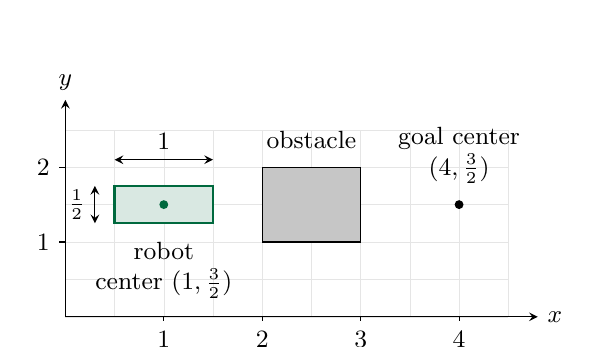
\begin{tikzpicture}[x=1.25cm,y=0.95cm,>=stealth,font=\small]
\draw[step=.5,gray!20,very thin] (0,0) grid (4.5,2.5);
\draw[->] (0,0)--(4.8,0) node[right] {$x$};
\draw[->] (0,0)--(0,2.9) node[above] {$y$};
\foreach \x in {1,2,3,4} \draw (\x,0)--(\x,-.06) node[below] {\x};
\foreach \y in {1,2} \draw (0,\y)--(-.06,\y) node[left] {\y};
\filldraw[fill=gray!45,draw=black] (2,1) rectangle (3,2);
\node[above] at (2.5,2.12) {obstacle};
\filldraw[fill=DartmouthGreen!15,draw=DartmouthGreen,thick]
 (.5,1.25) rectangle (1.5,1.75);
\fill[DartmouthGreen] (1,1.5) circle(1.6pt);
\node[below,align=center] at (1,1.13) {robot\\center $(1,\tfrac32)$};
\draw[<->] (.5,2.1)--node[above]{1}(1.5,2.1);
\draw[<->] (.3,1.25)--node[left]{$\tfrac12$}(.3,1.75);
\fill (4,1.5) circle(1.6pt);
\node[above,align=center] at (4,1.65) {goal center\\$(4,\tfrac32)$};
\end{tikzpicture}
\end{center}
\begin{enumerate}[label=(\alph*)]
\item Specify the configuration coordinates and the dimension of the
configuration space. If rotation were also allowed, what coordinate
would have to be added?
\begin{studentanswer}{2cm}
%%%%% SOLUTION HERE %%%%%

\end{studentanswer}
\item With the robot restricted to translation at the fixed orientation
shown, express the problem in configuration space and compute the set of
center positions for which the robot is in collision. Explain how
each of its four boundaries follows from the dimensions of the robot
and obstacle. Would checking the center against the original obstacle suffice?
\begin{studentanswer}{3cm}
%%%%% SOLUTION HERE %%%%%

\end{studentanswer}
\item Still without rotation, both center configurations
$(1,\tfrac32)$ and $(4,\tfrac32)$ are collision-free.
Is the straight-line motion between them valid?
Explain what this example requires a motion planner to check in addition
to the endpoints of an edge.
\begin{studentanswer}{2.3cm}
%%%%% SOLUTION HERE %%%%%

\end{studentanswer}
\end{enumerate}

\clearpage
\section*{Part 2: Programming}

The starter code is in \texttt{ps2/code/}. Task 1 implements gradient
descent.
Run \texttt{python ps2/code/autograder.py} from the repository root
to check the documented function interfaces.

\subsection{Task 1: gradient descent from scratch}

\textbf{Connection to Part 1.} P4 asks you to interpret learning-rate
behavior. This task implements gradient updates for a four-parameter model. P5 examines gradient steps on a local
quadratic approximation.

Implement the gradient and update directly, without automatic
differentiation or optimizer libraries. You will fit a degree-3 polynomial
$\hat{y}(x) = \theta_0 + \theta_1 x + \theta_2 x^2 + \theta_3 x^3$ to a
provided noisy 1D dataset (40 points from a smooth curve that is
\emph{not} a polynomial, so the fit cannot be perfect) by minimizing the
mean squared error
\[
\loss(\params) = \frac{1}{N}\sum_{i=1}^{N}\bigl(\hat{y}(x_i) - y_i\bigr)^2 .
\]

In \texttt{gd.py}, implement the loss, its analytic gradient with
respect to $\params$ (derive it on paper first, using the fact that the model is linear in
$\params$), and the gradient descent
loop $\params \leftarrow \params - \lr \nabla\loss(\params)$ that records
the loss at every iteration.

Then run the learning-rate experiment. Sweep $\lr$ over the four values in
the starter config, from small to large, and plot all four loss curves
on one set of axes with a log-scale $y$ axis. Deliver the plot of the
fitted curve against the data for your best $\lr$, the four-curve loss
plot, and three sentences classifying each $\lr$ (too small, well chosen,
too large but stable, diverging) with the evidence from your plot.

\textbf{Submission.} Put the four implementations in
\texttt{gd.py}. Put \texttt{ps2\_fit.png},
\texttt{ps2\_loss\_curves.png}, and your learning-rate classification in
the PDF response below.

\clearpage
\textbf{PDF responses.}
\begin{enumerate}[label=(\alph*)]

\item \begin{minipage}[t]{\linewidth}
Include \texttt{ps2\_fit.png}, showing the data and fitted polynomial for your selected learning rate.

\begin{studentanswer}{7cm}
%%%%% SOLUTION HERE %%%%%

\end{studentanswer}

\end{minipage}

\item \begin{minipage}[t]{\linewidth}
Include \texttt{ps2\_loss\_curves.png}, with all four learning rates labeled and a logarithmic loss axis.

\begin{studentanswer}{7cm}
%%%%% SOLUTION HERE %%%%%

\end{studentanswer}

\end{minipage}

\item \begin{minipage}[t]{\linewidth}
Classify the observed behavior of each learning rate and justify the classification using the curves.

\begin{studentanswer}{4cm}
%%%%% SOLUTION HERE %%%%%

\end{studentanswer}

\end{minipage}

\end{enumerate}

\docfooter
\end{document}
